%\documentclass[10pt]{beamer} 
\documentclass[10pt,xcolor=dvipsnames,mathserif]{beamer} 
\graphicspath{{figures/}}
\mode<presentation>
\useoutertheme{infolines} 
%\usetheme{CambridgeUS}
%\useoutertheme{infolines} 
\usetheme{Warsaw}
%\definecolor{MyColor}{rgb}{0.90,0.60,0}
%\usecolortheme{default}
%\setbeamercolor{itemize item}{fg=deepBlue}
%\setbeamercolor{section number projected}{bg=black,fg=yellow}
%\setbeamertemplate{headline}{}
\setbeamertemplate{headline}[infolines theme] 
%\setbeamertemplate{footline}[page number]
\setbeamertemplate{footline}[infolines theme] 
\setbeamertemplate{items}[ball] 
\setbeamertemplate{blocks}[rounded][shadow=true] 
\setbeamertemplate{navigation symbols}{} 

\usepackage{color}
%\usepackage{xcolor}
\usepackage{eulervm}
\usepackage[makeroom]{cancel}
\usepackage{mleftright}

\usepackage{blkarray}

%\setbeamercolor{structure}{fg=black!10!NavyBlue} 
\setbeamercolor{structure}{fg=blue!25!black} 
\setbeamercolor{foot1}{fg=white, bg=red!65!black} 
\setbeamercolor{foot2}{fg=white, bg=blue!25!black} 
\setbeamercolor{foot3}{fg=white, bg=red!65!black} 
%\setbeamertemplate{items}[ball] 
\setbeamertemplate{blocks}[rounded][shadow=true] 
\setbeamercolor{block body example}{bg=blue!25!white,fg=black}

%\logo{\includegraphics[height=1.0cm]{logo.png}}

\titlegraphic{
	\vskip-5mm
	%
\includegraphics[width=10mm]{logoAveiro.jpg}\hspace*{0.8cm}~%
	%
\includegraphics[width=30mm]{logoCIDMA.jpg}\hspace*{0.8cm}~%
	\hspace*{-0.5cm}
\includegraphics[width=28mm]{2017_FCT_H_cor.jpg}\hspace*{-0.5cm}~%
	%
\includegraphics[width=8mm]{logoLund.png}\hspace*{0.8cm}~
	
\includegraphics[width=75mm]{logoProj.jpeg}\hspace*{0.05cm}~
	
\includegraphics[width=25mm]{cost.jpg}
	%
	
}

%\makeatletter
%\setbeamertemplate{headline}
%{
%  \leavevmode%
%  \hbox{%
%  \begin{beamercolorbox}[wd=.5\paperwidth,ht=2.25ex,dp=1ex,right]{foot1}%
%    \usebeamerfont{author in head/foot}\insertsectionhead
%  \end{beamercolorbox}%
%  \begin{beamercolorbox}[wd=.01\paperwidth,ht=2.25ex,dp=1ex,center]{foot1}%
%    \usebeamerfont{title in head/foot}
%  \end{beamercolorbox}%
%  \begin{beamercolorbox}[wd=.01\paperwidth,ht=2.25ex,dp=1ex,center]{foot3}%
%    \usebeamerfont{title in head/foot}
%  \end{beamercolorbox}%
%  \begin{beamercolorbox}[wd=.5\paperwidth,ht=2.25ex,dp=1ex,left]{foot3}%
%    \usebeamerfont{date in head/foot}\insertsubsectionhead
%  \end{beamercolorbox}}%
%  \vskip2pt%
%}
%\makeatother

\makeatletter
\setbeamertemplate{footline}
{
  \leavevmode%
  \hbox{%
  \begin{beamercolorbox}[wd=.20\paperwidth,ht=2.25ex,dp=1ex,center]{foot1}%
    \usebeamerfont{author in head/foot}\insertshortauthor~~\beamer@ifempty{\insertshortinstitute}{}{(\insertshortinstitute)}
  \end{beamercolorbox}%
  \begin{beamercolorbox}[wd=.55\paperwidth,ht=2.25ex,dp=1ex,center]{foot2}%
    \usebeamerfont{title in head/foot}\insertshorttitle
  \end{beamercolorbox}%
  \begin{beamercolorbox}[wd=.25\paperwidth,ht=2.25ex,dp=1ex,right]{foot3}%
    \usebeamerfont{date in head/foot}\insertshortdate{}\hspace*{2em}
    \insertframenumber{} / \inserttotalframenumber\hspace*{2ex} 
  \end{beamercolorbox}}%
  \vskip0pt%
}
\makeatother

\usepackage{textpos} % package for the positioning
\usepackage{amsmath,amssymb,amsthm,mathrsfs,amsfonts,dsfont} 
\usepackage{graphicx}
%\usepackage[dvips]{graphicx}
%\usepackage{epsfig}
\usepackage{tabularx}
\usepackage{array}
\usepackage{colortbl}
\usepackage{cancel}
\usepackage{bm} % bold greek simbols
\usepackage{caption}
%\usepackage{subcaption}
\usepackage{verbatim}
\usepackage{hyperref}
\usepackage{fancybox}
\usepackage{bbold}
\usepackage{stackengine,mathtools}
\usepackage{booktabs}   % for fancy looking tables
\usepackage{multirow}


\usepackage{parskip}
% Our packages start
\usepackage{array}
\usepackage{multirow}   % analogue to \multicolumn
% Our packages end
\usepackage{multicol}
\usepackage{mleftright}
\usepackage[utf8x]{inputenc}
%\usepackage{slashed}
\usepackage{bbold}
%\usepackage{ulem}
%\usepackage[dvipsnames]{xcolor}
\usepackage{amscd}
\usepackage{placeins}
\usepackage{soul}
\usepackage{braket}
\usepackage{tikz-cd}
\usepackage{empheq}
\usepackage[most]{tcolorbox}
\usetikzlibrary{arrows, shapes,shadows}
\usepackage{mathtools,slashed}
\DeclareMathAlphabet{\mathpzc}{OT1}{pzc}{m}{it}
\usepackage{graphics}
\usepackage{arydshln}
\usepackage[english]{babel}
% or whatever

\usepackage{pifont}% http://ctan.org/pkg/pifont
\newcommand{\cmark}{\ding{51}}%
\newcommand{\xmark}{\ding{55}}%

%\usepackage[latin1]{inputenc}
% or whatever

\usepackage{times}
\usepackage[T1]{fontenc}
% Or whatever. Note that the encoding and the font should match. If T1
% does not look nice, try deleting the line with the fontenc.
\usepackage{graphicx}
\DeclareMathAlphabet{\mathpzc}{OT1}{pzc}{m}{it}

% Our definitions start

\newcommand{\ra}[1]{\renewcommand{\arraystretch}{#1}}
\newcommand*{\Scale}[2][4]{\scalebox{#1}{$#2$}}%
\newcommand\scalemath[2]{\scalebox{#1}{\mbox{\ensuremath{\displaystyle #2}}}}

\newcommand{\gev}{\,\textrm{GeV}}
\newcommand{\tr}{{\rm Tr}}
\newcommand{\del}{\partial}
\newcommand{\sgn}{\operatorname{sgn}}
\newcommand{\e}{\mathrm e}
\renewcommand{\d}{\mathrm d}
\renewcommand{\i}{\mathrm i}
\renewcommand{\(}{\left(}
\renewcommand{\)}{\right)}
\renewcommand{\[}{\left[}
\renewcommand{\]}{\right]}
\newcommand{\VSl}[3]{(\langle \tilde{L} \rangle ^{ #1} )^{ #2 }{}_{ #3 }}
\newcommand{\Sl}[3]{(\tilde{L}^{ #1} )^{ #2 }{}_{ #3 }}
\newcommand{\SlS}[3]{(\tilde{L}^*_{ #1} )_{ #2 }{}^{ #3 }}

\newcommand{\U}[1]{\mathrm{U}(1)_{\mathrm{#1}}}			% Use this for U(1) groups
\newcommand{\SU}[2]{\mathrm{SU}(#1)_{\mathrm{#2}}}		% Use this for SU(N) groups
\newcommand{\SO}[2]{\mathrm{SO}(#1)_{\mathrm{#2}}}		% Use this for SO(N) groups
\newcommand{\E}[1]{\mathrm{E}_{#1}}		% Use this for Exeptional groups
\newcommand{\T}[2]{T_{\mathrm{#1}}^{#2}}
\newcommand{\Q}[1]{\hat{Q}_{\mathrm{#1}}}				% Use this for generators	
\newcommand{\RN}[1]{%
	\textup{\uppercase\expandafter{\romannumeral#1}}%
}

% SUPERFIELDS
\newcommand{\LLR}[3]{\left(L^{ #1} \right)^{ #2 }{}_{ #3 }}
\newcommand{\QL}[3]{\left(Q_\mathrm{L}^{ #1} \right)^{ #2 }{}_{ #3 }}
\newcommand{\QR}[3]{\left(Q_\mathrm{R}^{ #1} \right)^{ #2 }{}_{ #3 }}

%FERMIONS
\newcommand{\LLRs}[3]{\left(L^*_{ #1} \right)_{ #2 }{}^{ #3 }}
\newcommand{\QLs}[3]{\left(Q^*_{\mathrm{L} #1} \right)_{ #2 }{}^{ #3 }}
\newcommand{\QRs}[3]{\left(\overline{Q}^*_{\mathrm{R} #1} \right)_{ #2 }{}^{ #3 }}


\newcommand{\FLLR}[3]{\big(L^{ #1} \big)^{ #2 }{}_{ #3 }}
\newcommand{\FQL}[3]{\big(Q_{\mathrm{L}}^{ #1} \big)^{ #2 }{}_{ #3 }}
\newcommand{\FQR}[3]{\big(Q_{\mathrm{R}}^{ #1} \big)^{ #2 }{}_{ #3 }}
\newcommand{\FDA}[2]{\Delta_{\mathrm{#1}}^{ #2}}

\newcommand{\FLLRd}[3]{\big(L^{\dagger}_{ #1} \big)_{ #2 }{}^{ #3 }}
\newcommand{\FQLd}[3]{\big(Q_{\mathrm{L}}^ {\dagger}{}_{ #1} \big)_{ #2 }{}^{ #3 }}
\newcommand{\FQRd}[3]{\big(Q_{\mathrm{R}}^{\dagger}{}_{ #1} \big)_{ #2 }{}^{ #3 }}
\newcommand{\FDAd}[2]{\Delta^{\dagger}_{\mathrm{#1}}{}^{ #2}}

%SCALARS
\newcommand{\SLLR}[3]{\left(\tilde{L}^{ #1} \right)^{ #2 }{}_{ #3 }}
\newcommand{\SQL}[3]{\left(\tilde{Q}_\mathrm{L}^{ #1} \right)^{ #2 }{}_{ #3 }}
\newcommand{\SQR}[3]{\left(\tilde{Q}_\mathrm{R}^{ #1} \right)^{ #2 }{}_{ #3 }}
\newcommand{\SLLRs}[3]{\left(\tilde{L}^*_{ #1} \right)^{ #3 }{}_{ #2 }}
\newcommand{\SQLs}[3]{\left(\tilde{Q}^*_{\mathrm{L} #1} \right)^{ #3 }{}_{ #2 }}
\newcommand{\SQRs}[3]{\left(\tilde{Q}^*_{\mathrm{R} #1} \right)_{ #3 }{}^{ #2 }}

\newcommand{\lam}[2]{\lambda_{\Scale[0.6]{#1 \-- #2}}}
\newcommand{\la}[1]{\lambda_{\Scale[0.6]{#1}}}
\newcommand{\lab}[1]{\bar{\lambda}_{\Scale[0.6]{#1}}}
\newcommand{\y}[1]{\mathrm{y}_{\Scale[0.6]{#1}}}
\newcommand{\mean}[1]{\left \langle #1 \right \rangle }
\newcommand{\vev}[1]{v_{\mathrm{#1}}}
\newcommand{\abs}[1]{\left| #1 \right| }
\newcommand{\g}[2]{g_{_\mathrm{#1}}^{#2}}

\newcommand{\blue}[0]{\color{blue}}
\newcommand{\green}[0]{\color{ForestGreen}}
\newcommand{\red}[0]{\color{red}}
\newcommand{\magenta}[0]{\color{magenta}}
\newcommand{\brown}[0]{\color{brown}}
\newcommand{\cyan}[0]{\color{cyan}}
\newcommand{\purple}[0]{\color{purple}}


\newcommand{\bfrac}[2]{\displaystyle\frac{#1}{#2}}
\newcommand{\conj}[1]{\ensuremath{#1^*}}
% Our definitions end

    \makeatletter
    \renewcommand*\env@matrix[1][*\c@MaxMatrixCols c]{%
      \hskip -\arraycolsep
      \let\@ifnextchar\new@ifnextchar
      \array{#1}}
    \makeatother

\title{How well can the muon $(g-2)_\mu$ anomaly be explained with a heavy $\U{B-L}$ $Z'$ gauge boson?}

\author[APM,RP] % (optional, for multiple authors)
{Ant\'onio~P.~Morais \inst{1} \and \textbf{João Pedro Rodrigues} \inst{1} \and Roman~Pasechnik \inst{2} \\ 
\vspace*{0.1cm}}

\institute[\tiny{AU,LU}]{
\inst{1} Center for Research and Development in Mathematics and Applications (CIDMA)\\ 
Aveiro University, Aveiro, Portugal \vspace*{0.1cm} \\
\inst{2} Department of Theoretical Physics, Lund University, Lund, Sweden \vspace*{-0.3cm}
}

\date[January 30th, 2021]{January 30th, 2021\vspace*{0.1cm}
\newline
Experiemnt vs Theory meeting $\--$ LIP Minho, Braga \vspace*{0.1cm}

}

\AtBeginSection[]
{
  \begin{frame}<beamer>
    \frametitle{Outline}
    \tableofcontents[currentsection]
  \end{frame}
}



\begin{document}

% Define block styles
\tikzstyle{block1} = [rectangle, draw, fill=blue!20, 
text width=18em, text centered, rounded corners, minimum height=4em, drop shadow]
\tikzstyle{block2} = [rectangle, draw, fill=blue!20, 
text width=28em, text centered, rounded corners, minimum height=4em, drop shadow]
\tikzstyle{block3} = [rectangle, draw, fill=blue!20, 
text width=26em, text centered, rounded corners, minimum height=4em, drop shadow]
\tikzstyle{block4} = [rectangle, draw, fill=blue!20, 
text width=22em, text centered, rounded corners, minimum height=4em, drop shadow]
\tikzstyle{block5} = [rectangle, draw, fill=blue!20, 
text width=16em, text centered, rounded corners, minimum height=4em, drop shadow]
\tikzstyle{block6} = [rectangle, draw, fill=blue!20, 
text width=12em, text centered, rounded corners, minimum height=4em, drop shadow]
\tikzstyle{line} = [draw, -latex']
\tikzstyle{cloud} = [draw, ellipse,fill=red!20, node distance=3cm,
minimum height=2em]


\begin{frame}
  \titlepage
\end{frame}


%\begin{frame}{Take home message}
%	
%	\begin{exampleblock}{}
%		{\bf Explore the {\blue origin} of the observed particle spectrum in Nature from {\blue unification principles} and which new physics phenomena are expected.}
%	\end{exampleblock}
%	
%\end{frame}


 \begin{frame}
   \frametitle{Outline}
   \tableofcontents
%   % You might wish to add the option [pausesections]
 \end{frame}



\section{Introduction}

\begin{frame}{Introduction}
	
\textbf{Motivations for $\bm{\mathrm{B-L}}$ (Baryon number minus Lepton number) symmetry:}
\vskip5mm
\begin{itemize}
	\item The SM contains an accidental symmetry that conserves $\mathrm{B-L}$,
	\vskip2mm
	\item $\mathrm{B-L}$ symmetry relevant for baryogenesis through leptogenesis,
	\begin{itemize}
		\item[>] sphaleron process violates $\mathrm{B}$ but preserves $\mathrm{B-L}$
	\end{itemize}  
	\item Grand Unified Theories, e.g.~$\SO{10}{}$, $\E{6}$, $\E{8},\ldots$ contain gauged $\U{B-L}$,
	\vskip2mm
	\item The scale of $\U{B-L}$ breaking sets the mass scale of the right-handed Majorana neutrinos.
\end{itemize}
				
\end{frame}


\begin{frame}{BSM physics}
	
		\begin{itemize}
			\item \textbf{Three} generations of right-handed neutrinos $\to$ \textbf{\red no gauge anomalies}
			\begin{itemize}
				\item[>] Lightest is sterile and can be keV to TeV dark matter candidate. \\ {\blue \scriptsize  Kaneta, Kang, Lee: JHEP 1702 (2017) 031}
				\item[>] Or stabilized via a $\mathbb{Z}_2^{\mathrm{DM}}$
				\begin{itemize}
					\item[-] Annihilation via $Z^\prime$ portal {\scriptsize \blue Okada: Adv.High Energy Phys. 2018 (2018) 5340935}
					\item[-] Annihilation via Higgs portal {\scriptsize  \blue Okada, Seto: Phys.Rev. D82 (2010) 023507}
					\end{itemize}
			\end{itemize}
			\vskip2mm
			\item Model contains a complex-singlet scalar $\chi$ whose VEV breaks $\U{B-L}$
			\begin{itemize}
				\item[>] Scalar sector studies: {\scriptsize  \blue Basso, Moretti, Pruna: Eur.Phys.J. C71 (2011) 1724, Phys.Rev. D82 (2010) 055018}
				\vskip2mm
				\item[>] Enhanced vacuum stability compared to the SM
				
		\end{itemize}	
			\vskip2mm
			\item Model contains an extra $Z^\prime$ gauge boson {\scriptsize  \blue Basso, Belyaev, Moretti, Pruna: JHEP 0910 (2009) 006} ; {\scriptsize  \blue Basso, Belyaev, Moretti, Shepherd-Themistocleous: Phys.Rev. D80 (2009) 055030}
%			\begin{itemize}
%				\item[>] \textbf{BSM vector bosons contribute to $\bm{\(g-2\)_\mu}$ anomaly}
%				%%%%%%%%%%%%%%%%%%%%%%%%%
%				\begin{figure}[!h]
%					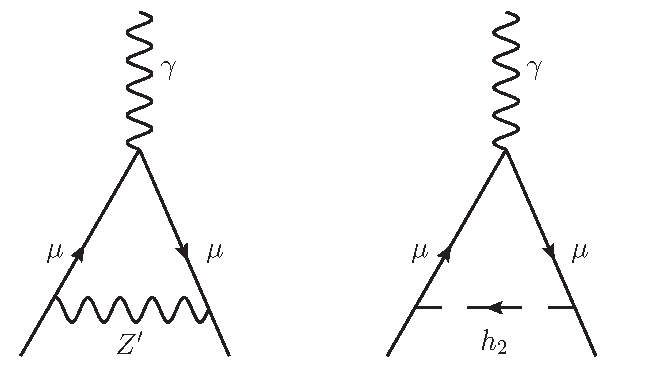
\includegraphics[scale=0.4]{g-2.pdf}
%				\end{figure}	
%				%%%%%%%%%%%%%%%%%%%%%%%%%
%				\item[>] {\bf \red Not studied in the B-L SM} (recently addressed in the B-L SSM \\ {\scriptsize \blue Yang, Feng et al. Phys.Rev. D99 (2019) no.1, 015002})
%			\end{itemize}
			 
		\end{itemize}
		
	
\end{frame}

\begin{frame}
	
			\begin{exampleblock}{}
				{\bf BSM vector bosons and scalars
					 contribute to $\bm{\(g-2\)_\mu}$ anomaly }
			\end{exampleblock} 
		%%%%%%%%%%%%%%%%%%%%%%%%%
		\begin{figure}[!h]
			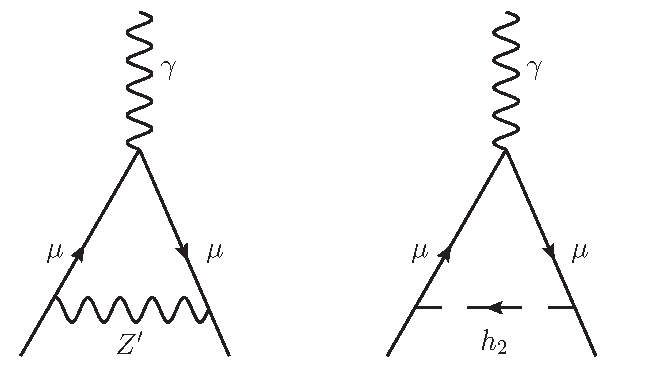
\includegraphics[scale=0.6]{g-2.pdf}
		\end{figure}	
		%%%%%%%%%%%%%%%%%%%%%%%%%			
		{\bf \red Not studied in the B-L SM} (recently discussed in the supersymmetric version B-L SSM {\scriptsize \blue Yang, Feng et al. Phys.Rev. D99 (2019) no.1, 015002})

\end{frame}

\begin{frame}
	Direct $Z^\prime$ searches exclude masses below $m_{Z^\prime} \approx 4~\mathrm{TeV}$ {\scriptsize \blue ATLAS-CONF-2017-027} 
		%%%%%%%%%%%%%%%%%%%%%%%%%
		\begin{figure}[!h]
			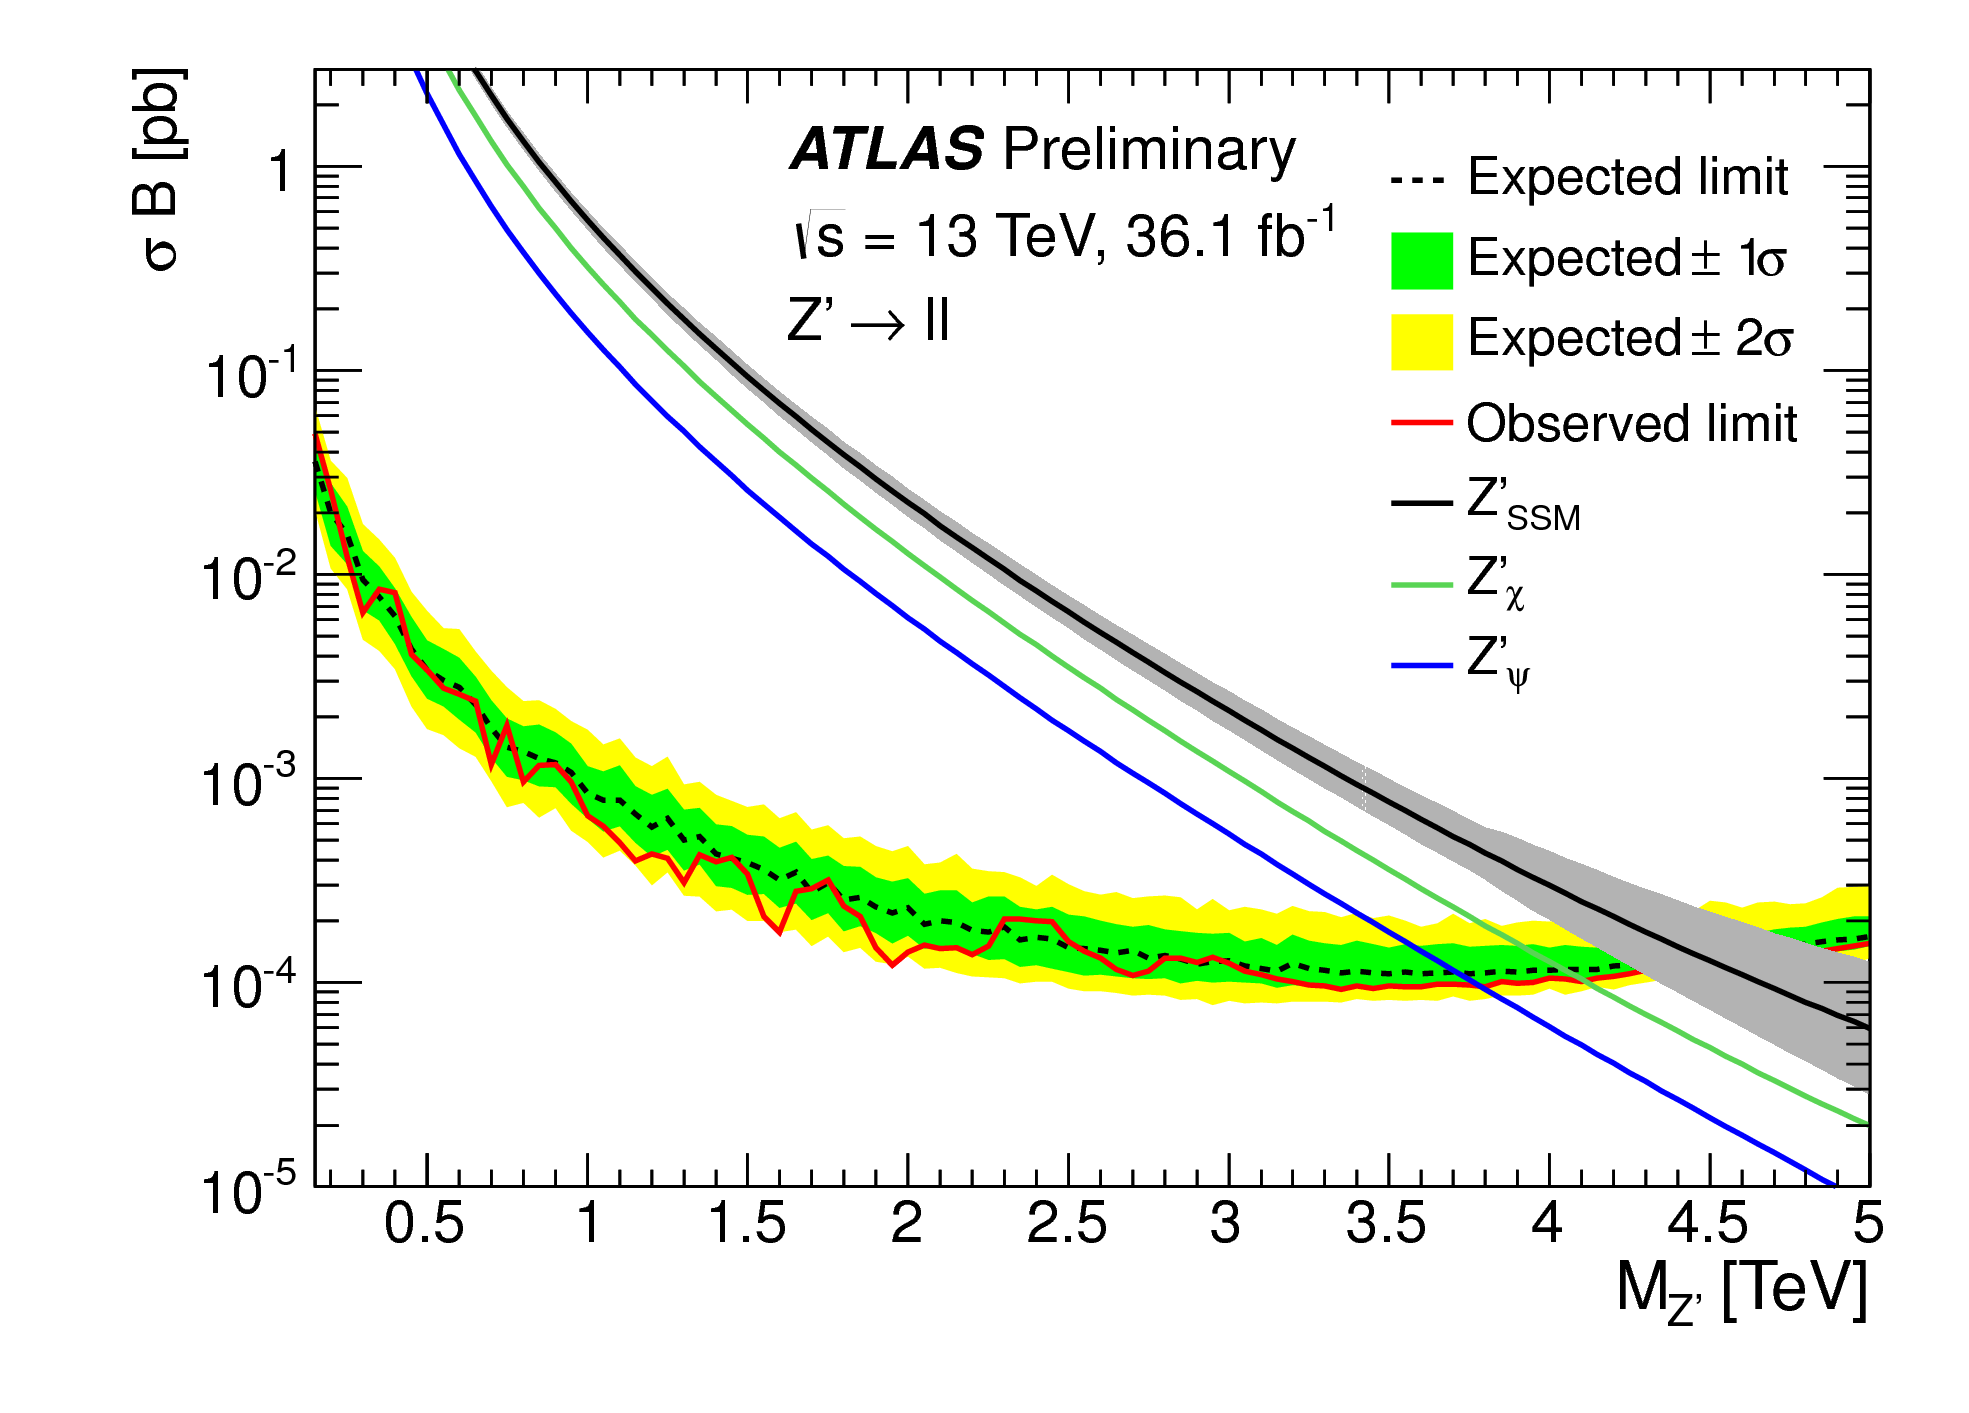
\includegraphics[scale=0.12
			]{fig_04.png}
		\end{figure}	
		%%%%%%%%%%%%%%%%%%%%%%%%%
		
\begin{itemize}
	\item Can the minimal B-L SM still address the muon $\(g-2\)_\mu$ anomaly and how well? 
\end{itemize}		
		
\end{frame}


\section{The minimal $\U{B-L}$ extension of the SM}

\begin{frame}{The minimal $\U{B-L}$ extension of the SM}
	
%
\begin{table}[htb!]
	\begin{center}
		\begin{tabular}{ccccc}
			\toprule                     
			& $\SU{3}{C}$ & $\SU{2}{L}$ & $\U{Y}$ & $\U{B-L}$  	\\    
			\midrule
			$q_\mathrm{L}$     			    							& $\bm{3}$		& $\bm{2}$	&	$1/6$ & $1/3$	\\
			$u_\mathrm{R}$     			    							& $\bm{3}$		& $\bm{1}$	&	$2/3$ & $1/3$	\\
			$d_\mathrm{R}$     			    							& $\bm{3}$		& $\bm{1}$	&	$-1/3$ & $1/3$	\\
			$\ell_\mathrm{L}$     			    							& $\bm{1}$		& $\bm{2}$	&	$-1/2$ & $-1$	\\
			$e_\mathrm{R}$     			    							& $\bm{1}$		& $\bm{1}$	&	$-1$ & $-1$	\\
			$\nu_\mathrm{R}$     			    							& $\bm{1}$		& $\bm{1}$	&	$0$ & $-1$	\\
			\hdashline
			$H$     			    							& $\bm{1}$		& $\bm{2}$	&	$1/2$ & $0$	\\
			$\chi$     			    							& $\bm{1}$		& $\bm{1}$	&	$0$ & $2$	\\
			\bottomrule
		\end{tabular} 
	%	\caption{\it{Charge assignment of the singlets, doublets and bi-doublets under the accidental symmetries. All three families are implicit.}}
	%	\label{tab:AccSym}  
	\end{center}
\end{table} 
%


	
\end{frame}

\begin{frame}{Scalar sector}
	
		\begin{equation*}
		\label{eq:potential}
		V(H,\chi)= m^2 H^\dagger H + \mu^2 \chi^\ast \chi + \lambda_1 (H^\dagger H)^2 + \lambda_2 \(\chi^\ast \chi\)^2 + \lambda_3  \chi^\ast \chi H^\dagger H
		\end{equation*}
		
				
		\begin{itemize}
			 \item Boundedness from below: $4 \lambda_1 \lambda_2 - \lambda_3^2 >0$ and $\lambda_1,\lambda_2 > 0$
		\end{itemize}
		
	\begin{equation*}
	\begin{aligned}
	H = \dfrac{1}{\sqrt{2}} 
		\begin{pmatrix}
		-i \(\omega_1 - i \omega_2 \) \\
		v + (h + i z)
		\end{pmatrix}	
		\qquad
		\chi = \dfrac{1}{\sqrt{2}} \[ x + \(h^\prime + i z^\prime\) \]	
	\end{aligned}
	\end{equation*}	

		\begin{itemize}
			\item $\omega^\pm = \omega_1 \mp i \omega_2$, $z$ and $z^\prime$ are Goldstone bosons eaten by $W^\pm$, $Z$ and $Z^\prime$
		\end{itemize}		
		\begin{equation*}
		\begin{aligned}
		\mean{H} = \dfrac{1}{\sqrt{2}} 
		\begin{pmatrix}
		0 \\
		v 
		\end{pmatrix}	
		\qquad
		\mean{\chi} = \dfrac{x}{\sqrt{2}}
		\qquad \Rightarrow \qquad
		\begin{cases}
		v^2 = \tfrac{-\lambda_2 m^2 + \tfrac{\lambda_3}{2}\mu^2}{\lambda_1 \lambda_2 - \tfrac{1}{4}\lambda_3^2} > 0\\
		x^2 = \tfrac{-\lambda_1 \mu^2 + \tfrac{\lambda_3}{2}m^2}{\lambda_1 \lambda_2 - \tfrac{1}{4}\lambda_3^2} > 0
		\end{cases}	
		\end{aligned}
		\end{equation*}			
		
\end{frame}

%%%%%%%%%%%%%%%%%%%%%%%%%%%%%

\begin{frame}
	
	\begin{columns}
		\column{.5\textwidth}
		\begin{equation*}
		\begin{aligned}
		\begin{cases}
		\lambda_2 m^2 < \tfrac{\lambda_3}{2} \mu^2 \\
		\lambda_1 \mu^2 < \tfrac{\lambda_3}{2} m^2 \\
		4 \lambda_1 \lambda_2 - \lambda_3^2 >0 \\
		\lambda_1,\lambda_2 > 0
		\end{cases}	
		\end{aligned}
		\end{equation*}
		\column{.5\textwidth}
		\begin{itemize}
			\item[] \xmark: There is no solution
			\item[] \checkmark: There is solution
		\end{itemize}
		
	\end{columns}
						
	%
	\begin{table}[htb!]
		\begin{center}
			\begin{tabular}{ccccc}
				\toprule                     
				& $\mu^2 > 0$ & $\mu^2 > 0$ & $\mu^2 < 0$ & {\red $\mu^2 < 0$}  	\\
				& $m^2 > 0$ & $m^2 < 0$ & $m^2 > 0$ & {\red $m^2 < 0$}  	\\        
				\midrule
				$\lambda_3 < 0 $     			    							& \xmark		& \checkmark	&	\checkmark & {\red \checkmark}	\\
				& 		& 	&	 & 	\\
				$\lambda_3 > 0$     			    							& \xmark		& \xmark	&	\xmark & {\red \checkmark}	\\
				\bottomrule
			\end{tabular} 
			%	\caption{\it{Charge assignment of the singlets, doublets and bi-doublets under the accidental symmetries. All three families are implicit.}}
			%	\label{tab:AccSym}  
		\end{center}
	\end{table} 
	%
%\pause
\vskip3mm
	\begin{equation*}
	\begin{aligned}
	\begin{pmatrix}
	h_1 \\
	h_2 
	\end{pmatrix}
	=
	\begin{pmatrix}
	\cos \alpha_h & -\sin \alpha_h \\
	\sin \alpha_h & \cos \alpha_h 
	\end{pmatrix}
	\begin{pmatrix}
	h \\
	h^\prime 
	\end{pmatrix}
	\end{aligned}
	\end{equation*}
	\vskip0.1mm
	{\bf Heavy $Z^\prime$ implies that $\bm{x \gg v}$ for most of the parameters points:}
	\begin{equation*}
	\sin \alpha_h \approx \dfrac{1}{2}\dfrac{\lambda_3}{\lambda_2} \dfrac{v}{x} \qquad
		m_{h_1}^2 \approx 2 \lambda_1 v^2 \qquad m_{h_2}^2 \approx 2 \lambda_2 x^2
	\end{equation*}

\end{frame}

\begin{frame}{Gauge Kinetic Mixing}
	
		\begin{equation*}
		\begin{aligned}
		\mathcal{L}_\mathrm{bosons} =  \abs{D_\mu H}^2 + \abs{D_\mu \chi}^2 - V\(H,\chi\) -\dfrac{1}{4} F_{\mu \nu} F^{\mu \nu} -\dfrac{1}{4} F^\prime_{\mu \nu} F^{\prime \mu \nu} -\dfrac{1}{2} \kappa F_{\mu \nu} F^{\prime \mu \nu}
		\end{aligned}
		\end{equation*}
	
			\begin{itemize}
				\item $\kappa$ is a ${\green \U{Y}} \times {\red \U{B-L}}$ gauge
				kinetic-mixing parameter
				\vskip2mm
				\item Field strength tensors ${\green F_{\mu \nu} = \partial_\mu A_\nu - \partial_\nu A_\mu}$ and ${\red F^\prime_{\mu \nu} = \partial_\mu A^\prime_\nu - \partial_\nu A^\prime_\mu}$
				\item {\blue Redefine $\kappa = \sin \alpha$ and gauge fields as (convenient basis choice)}
				\begin{equation*}
				\begin{pmatrix}
				A_\mu \\
				A^\prime_\mu 
				\end{pmatrix}
				=
				\begin{pmatrix}
				1 & -\tan \alpha \\
				0 & \sec \alpha 
				\end{pmatrix}
				\begin{pmatrix}
				B_\mu \\
				B^\prime_\mu 
				\end{pmatrix}\,,
				\label{eq:trans-kappa}
				\end{equation*}	
				\item Kinetic terms acquire canonical form
				\begin{equation*}
				\begin{aligned}
				\mathcal{L}_\mathrm{kinetic} =   -\dfrac{1}{4} B_{\mu \nu} B^{\mu \nu} -\dfrac{1}{4} B^\prime_{\mu \nu} B^{\prime \mu \nu}
				\end{aligned}
				\end{equation*}					
			\end{itemize}
			
	
\end{frame}

\begin{frame}
	
	
	\textbf{Redefined covariant derivative absorbs the kinetic mixing information:}
	
	\begin{equation*}
	\begin{aligned}
	D_\mu = \partial_\mu + i \(g_Y \; Y + g_{BY} \; Y_{B-L}\) B_\mu + i \(g_{BL} \; Y_{B-L} + g_{YB} \; Y\) B_\mu^\prime
	\end{aligned}
	\end{equation*}	
	\vskip2mm
	\begin{itemize}
		\item $g_1$ and $g_1^\prime$ are $\U{Y}$ and $\U{B-L}$ gauge couplings
		\vskip2mm
		\item $g_{YB}$ and $g_{BY}$ result from the kinetic mixing
\vskip2mm
		\item With our basis choice
		 $$\begin{cases}
				g_Y = g_1 \\
				{\blue g_{BL} = g_1^\prime \sec \alpha} \\
				{\red g_{YB} = -g_1 \tan \alpha }\\
			    g_{BY} = 0
		\end{cases} 
		\qquad
		\text{No mixing limit:}\quad \sec \alpha = 1 \Rightarrow {\blue g_{BL} = g_1^\prime}$$
	\end{itemize}

\end{frame}

\begin{frame}
	\begin{exampleblock}{}
		{\bf Gauge kinetic-mixing induces mixing between $Z^\prime$, $Z$ and $\gamma$ }
	\end{exampleblock} 
	
	\begin{equation*}
	\begin{aligned}
	\begin{pmatrix}
	\gamma_\mu \\
	Z_\mu \\
	Z^\prime_\mu
	\end{pmatrix}
	=
	\begin{pmatrix}
	\cos \theta_W & \sin \theta_W & 0\\
	-\sin \theta_W \cos \theta_W^\prime & \cos \theta_W \cos \theta_W^\prime & \sin \theta_W^\prime \\
	\sin \theta_W \sin \theta_W^\prime & -\cos \theta_W^\prime \sin \theta_W^\prime & \cos \theta_W^\prime
	\end{pmatrix}
	\begin{pmatrix}
	B_\mu \\
	A^3_\mu \\
	B^\prime_\mu
	\end{pmatrix}
	\end{aligned}
	\end{equation*}	
	$$ \text{Again in the limit $x \gg v$ \qquad } \sin \theta_W^\prime \approx \dfrac{1}{8
		} \dfrac{g_{YB}}{g_{BL}}\(\dfrac{v}{x}\)^2 \sqrt{g^2 + g_Y^2}$$
	\begin{itemize}
		\item $g$ is $\SU{2}{L}$ gauge coupling
		\vskip2mm
		\item $\sin \theta_W^\prime = 0$ for no kinetic mixing, $g_{YB} = 0$, and {\red $Z_\mu^\prime = B_\mu^\prime$}
		\begin{itemize}
			\item[>] For $g_{YB} = 0$ we have $m_Z = \tfrac{1}{2} v \sqrt{g^2 + g_Y^2}$ and ${\red m_{Z^\prime} \approx 2 g_{BL} x}$
			\item[>] For $x \gg v$ we also have ${\red m_{Z^\prime} \approx 2 g_{BL} x}$
		\end{itemize}
	\end{itemize}
	
\end{frame}

\begin{frame}{Yukawa sector}
	\begin{equation*}
	\begin{aligned}
	\mathcal{L}_\mathrm{Yukawa} = 
	-y_u^{ij} \overline{q_\mathrm{L i}} u_\mathrm{R j} \widetilde{H} 
	-y_d^{ij} \overline{q_\mathrm{L i}} d_\mathrm{R j} H
	-y_e^{ij} \overline{\ell_\mathrm{L i}} e_\mathrm{R j} H
	{\red - y_\nu^{ij} \overline{\ell_\mathrm{L i}} \nu_\mathrm{R j} \widetilde{H}
		-\dfrac{1}{2} y_M^{ij} \overline{\nu_\mathrm{R i}^c} \nu_\mathrm{R j} \chi} + \mathrm{c.c.}
	\end{aligned}
	\end{equation*}
	\begin{itemize}
		\item $\widetilde{H} = i \sigma^2 H^*$
		\vskip2mm
		\item Dirac and Majorana masses matrices: $\bm{m_D} = \tfrac{\bm{y_\nu}}{\sqrt{2}} v$ and $\bm{M} = \tfrac{\bm{y_M}}{\sqrt{2}} x$
		\item Neutrino masses via see-saw mechanism: $\begin{pmatrix}
		0 & m_D \\
		m_D & M\\
		\end{pmatrix} \rightarrow 
		\begin{cases}
		m_{\nu_l} \approx \tfrac{m_D^2}{M}\\
		m_{\nu_h} \approx M
		\end{cases}$
		\item Small mixing angle: $\tan \alpha_\nu \approx -2 \sqrt{\tfrac{m_{\nu_l}}{m_{\nu_h}}}$
	\end{itemize}
	
\end{frame}

\section{Results}

\begin{frame}{Results}
		%
		\begin{table}[htb!]
			\begin{center}
				\begin{tabular}{ccccc}
					\toprule                     
				 $\lambda_1$ & $\lambda_{2,3}$ & $g_{BL}$ & $g_{YB}$ & $x~\mathrm{[TeV]}$  
				 \\       
					\midrule
				$\[10^{-2},\; 10^{0.5}
				\]$	& $\[10^{-8},\; 10
					\]$ 			    							& $\[10^{-8},\; 3
					\]$		& $\[10^{-8},\; 3
					\]$	&	$\[0.5,\; 20.5
					\]$ 	\\
					\bottomrule
				\end{tabular}  
			\end{center}
		\end{table} 
		%
		\begin{enumerate}
			\item Model file: \texttt{SARAH-4.12.3}
			\item Spectrum generator: \texttt{SPheno-4.0.3}
			\begin{itemize}
				\item Unitarity
				\item One-loop mass spectrum and two-loop Higgs mass
				\item Mixing angles
				\item EW precision observables STU
				\item $\(g-2\)_\ell$
				\item Decay widths and Branching Fractions
			\end{itemize}
			\item Generated points with $m_{h_1} = 125.2 \pm 2~\mathrm{GeV}$ input to \texttt{HiggsBounds-4.3.1} and  \texttt{HiggsSingnals-1.4.0}
			\item \textbf{Surviving} points passed to \texttt{MadGraph5$\_$am5@NLO}
		\end{enumerate}
		
\end{frame}

\begin{frame}

		%%%%%%%%%%%%%%%%%%%%%%%%%
\begin{figure}[!htb]
	\centering
	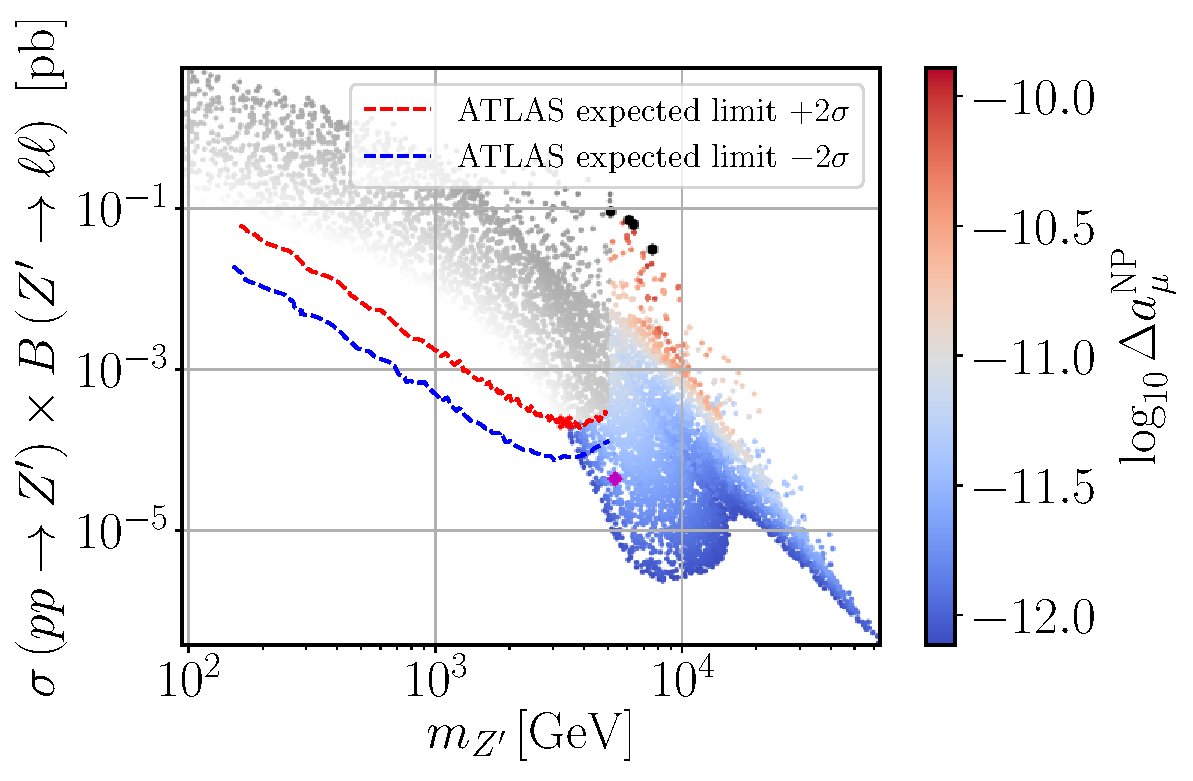
\includegraphics[scale=0.27]{mZp_Xsec_Amu.pdf}
	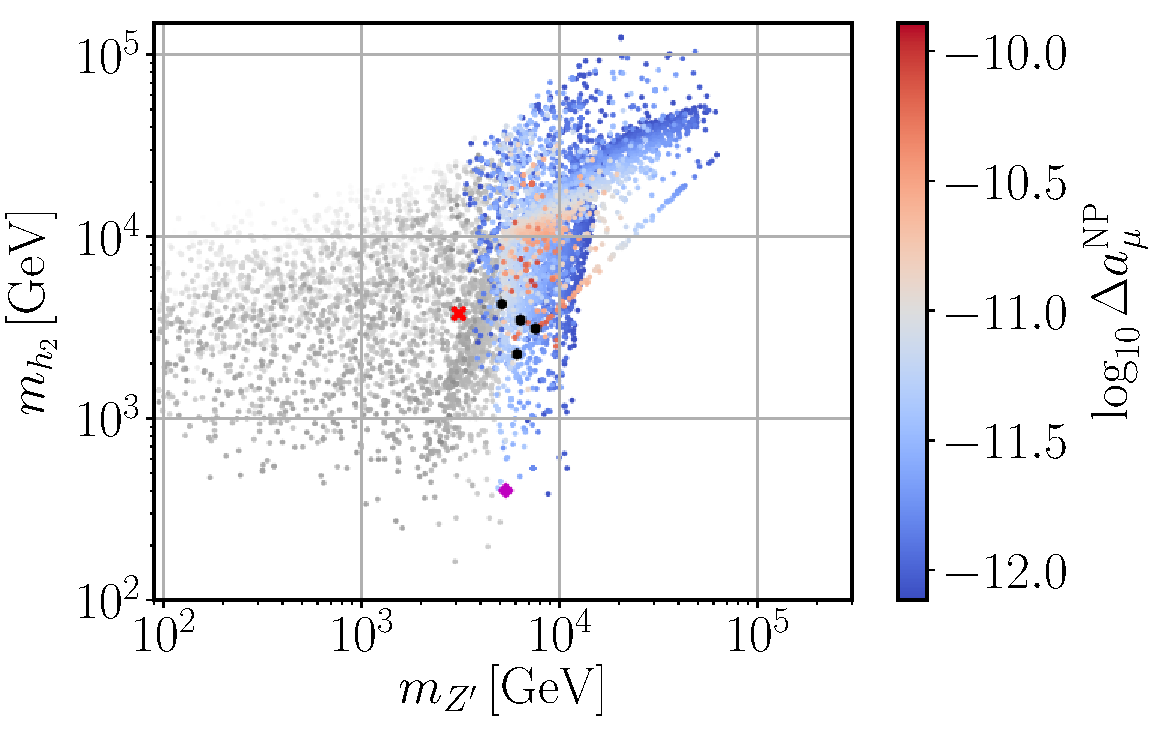
\includegraphics[scale=0.27]{mZp_Mhp_Amu.pdf}
\end{figure}		
		%%%%%%%%%%%%%%%%%%%%%%%%%
		\vskip-2mm
		\begin{itemize}
			\item Applied LEP constraints from 4 fermion contact interactions
			\vskip2mm
			\item {\bf Model explains $\bm{\(g-2\)_\mu}$ for $\bm{5~\mathrm{TeV} \lesssim m_{Z^\prime} \lesssim 8~\mathrm{TeV}}$ within $-2.25\sigma$ uncertainty (4 black dots).}
			\vskip2mm
			\item Red cross highlights a benchmark point with $m_{Z^\prime} \approx 3~\mathrm{TeV}$ regarded as an early-discovery (or early-exclusion) scenario in future LHC runs.
			\vskip2mm
			\item Magenta diamond corresponds to the lightest BSM Higgs found, $m_{h_2} \approx 396~\mathrm{GeV}$
		\end{itemize}
	
\end{frame}

\begin{frame}
$\Delta a_\mu^{Z^\prime}$ calculated in \texttt{SARAH} and numerically evaluated in \texttt{SPheno}
			\vskip2mm				
\begin{itemize}
	\item When $\tfrac{m_\mu}{m_{Z^\prime}} \ll 1 $ the $Z'$ contribution reads
\end{itemize}
				\begin{equation*}
				\Delta a_\mu^{Z^\prime} \approx -\tfrac{1}{3 \pi^2} \tfrac{m_\mu^2}{m_{Z^\prime}^2} \[6 \g{L}{\mu \mu Z^\prime} \g{R}{\mu \mu Z^\prime} - 4 \({\g{L}{\mu \mu Z^\prime}}^2 + {\g{R}{\mu \mu Z^\prime}}^2\) \]\,
				\end{equation*}
			%\vskip-2mm
Contribution from $h_2$ is tiny: $\Delta a_\mu^{h_2} \propto \tfrac{m_\mu^2}{m_{h_2}^2}\(y_\mu \sin \alpha_h\)^2$
\vskip-2mm
%%%%%%%%%%%%%%%%%%%%%%%%%
\begin{figure}[!h]
	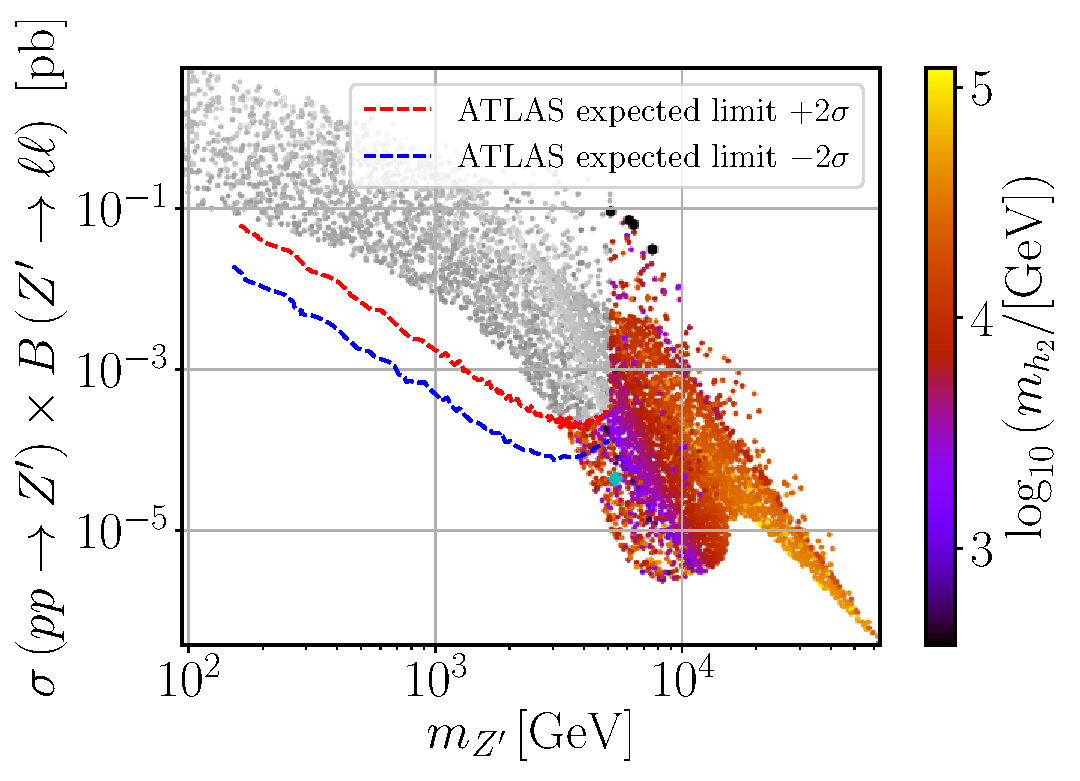
\includegraphics[scale=0.28
	]{mZp_Xsec_mh2.pdf}\qquad
	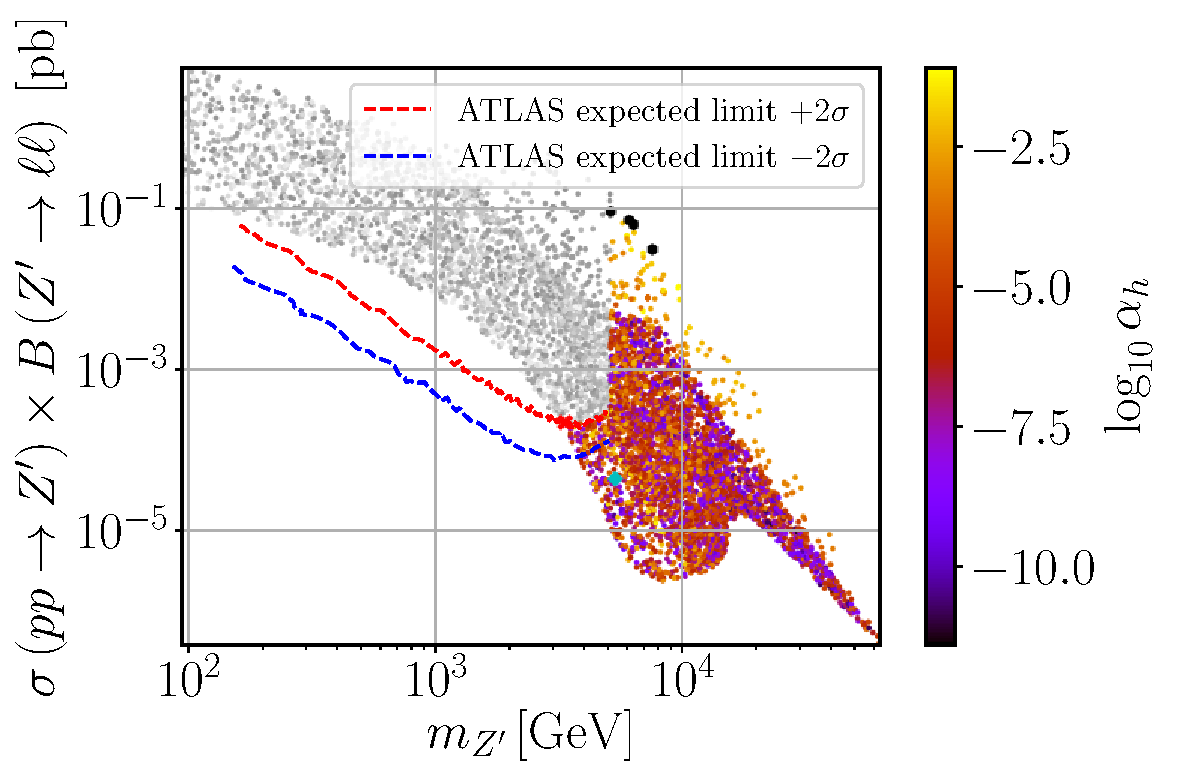
\includegraphics[scale=0.28
	]{mZp_Xsec_alpha.pdf}
\end{figure}	
%%%%%%%%%%%%%%%%%%%%%%%%%
Suppressed by $\sin^2 \alpha_h < 0.0064$ and $m_{h_2} > 396~\mathrm{GeV}$
\end{frame}

\begin{frame}
Expanding for $v \ll x$
$$\g{L}{\ell \ell Z^\prime} \simeq \g{B-L}{} + \dfrac{1}{2} \g{YB}{}\,,
\qquad
\g{R}{\ell \ell Z^\prime} \simeq \g{B-L}{} + \g{YB}{}\,.$$
\vskip-5mm
%%%%%%%%%%%%%%%%%%%%%%%%%
\begin{figure}[!h]
	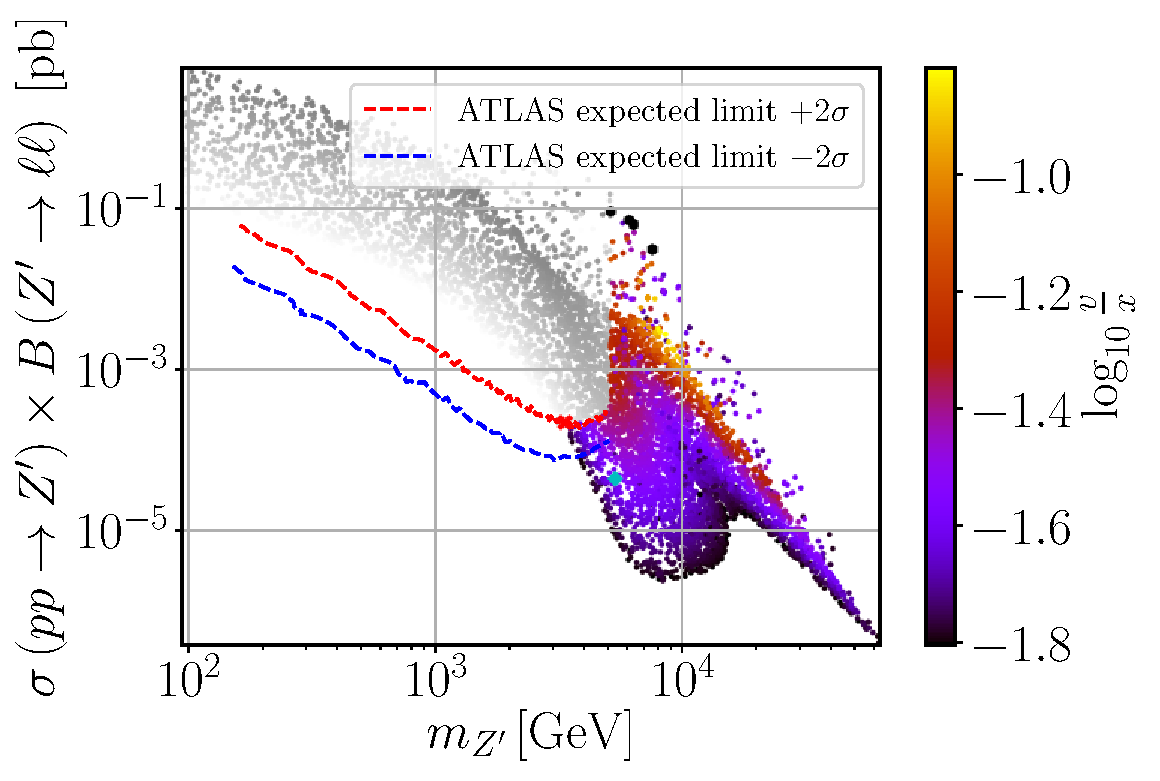
\includegraphics[scale=0.35
	]{mZp_Xsec_VEV.pdf}
\end{figure}	
%%%%%%%%%%%%%%%%%%%%%%%%%
$$\Delta a_\mu^{Z^\prime} \simeq \dfrac{1}{3 \pi^2} {\red \dfrac{m_\mu^2}{m_{Z^\prime}^2}} \[2\(g_{_\mathrm{B-L}}^{2} + g_{_\mathrm{YB}}^{2}\) + 3 g_{_\mathrm{B-L}}^{} g_{_\mathrm{YB}}^{} \]$$
\textbf{To enhance $\Delta a_\mu^{Z^\prime}$ for heavy $Z'$ one needs sizeable $g_{_\mathrm{B-L}}$ and/or $g_{_\mathrm{YB}}$}
\begin{itemize}
	\item Note strong correlation between $\red v/x$ and $\Delta a_\mu^{Z^\prime}$ except for the sparser upper edge!
\end{itemize}
\end{frame}

\begin{frame}
	Four-fermion contact interactions constrain $\g{B-L}{} < 1.8$ in the B-L SM
	%%%%%%%%%%%%%%%%%%%%%%%%%
	\begin{figure}[!h]
		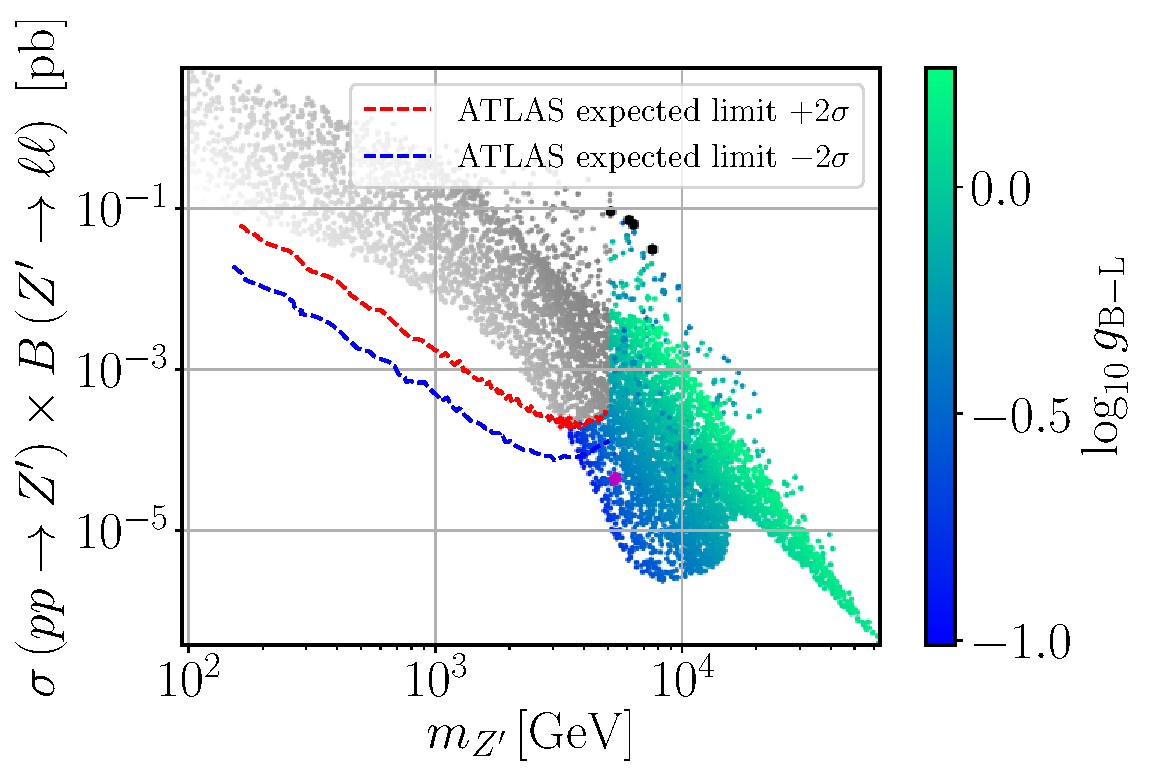
\includegraphics[scale=0.27
		]{mZp_Xsec_gBL.pdf}~
		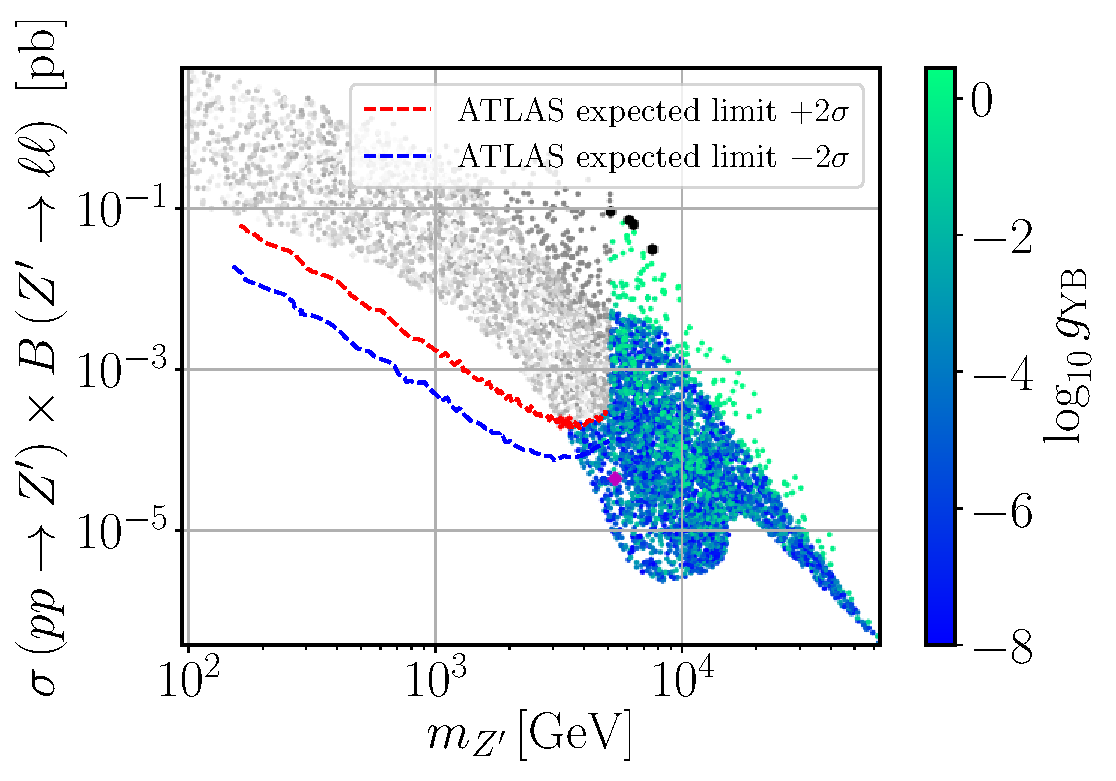
\includegraphics[scale=0.27
		]{mZp_Xsec_gYB.pdf}
	\end{figure}	
	%%%%%%%%%%%%%%%%%%%%%%%%%
	Enhancement of $\Delta a_\mu^{Z^\prime}$ is due to sizeable $\g{YB}{}$, thus large $\g{L,R}{\ell \ell Z'}$
	%%%%%%%%%%%%%%%%%%%%%%%%%
\begin{figure}[!h]
	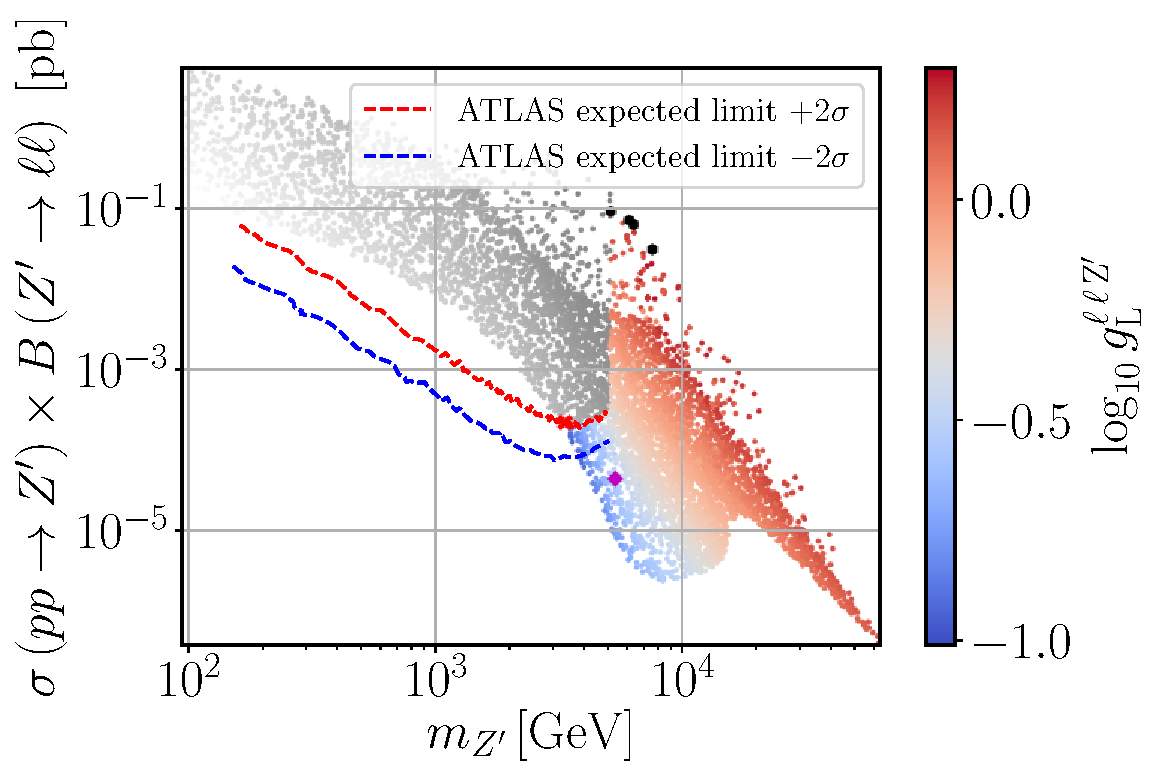
\includegraphics[scale=0.27
	]{mZp_Xsec_gLmumuZ.pdf}~
	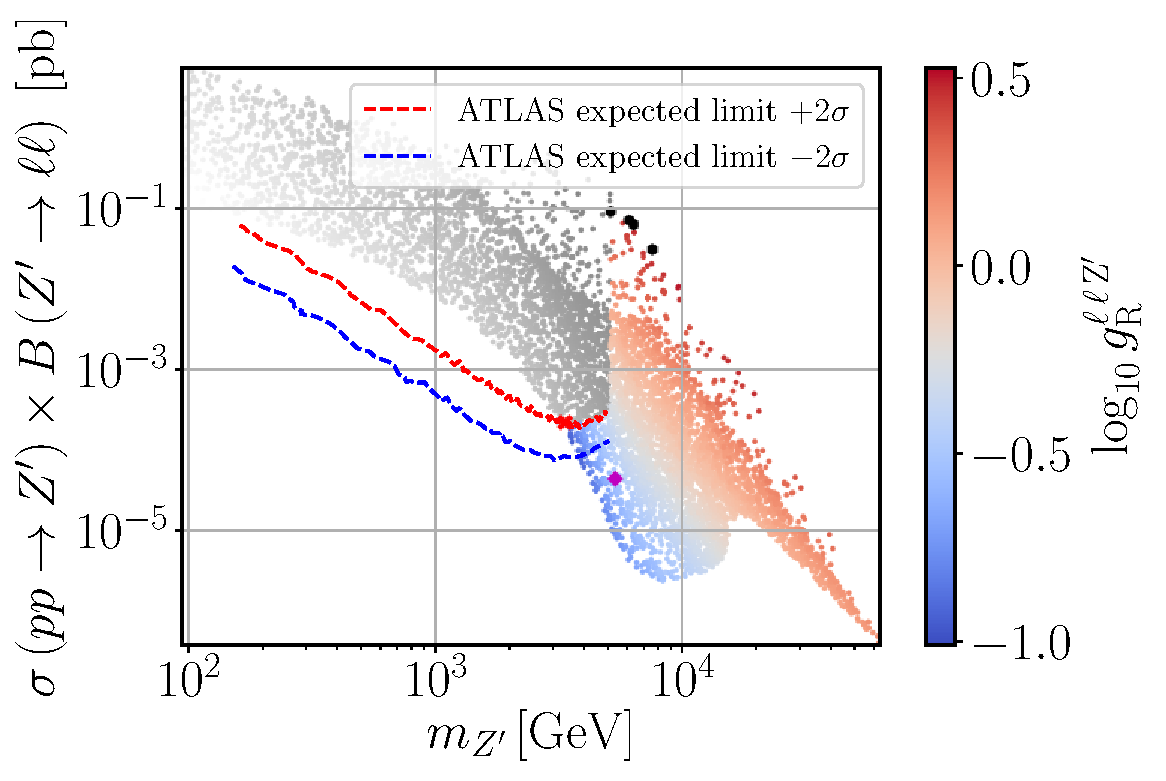
\includegraphics[scale=0.27
	]{mZp_Xsec_gRmumuZ.pdf}
\end{figure}	
%%%%%%%%%%%%%%%%%%%%%%%%%	
\end{frame}

\begin{frame}
	LEP constraints set upper bound $\sin \theta_W^\prime \lesssim 10^{-3}$
	$$\sin \theta_W^\prime \approx \dfrac{1}{8
	} \dfrac{g_{YB}}{g_{BL}}\(\dfrac{v}{x}\)^2 \sqrt{g^2 + g_Y^2}$$
which is respected even for the larger values of $\g{YB}{}$:	%%%%%%%%%%%%%%%%%%%%%%%%%
\begin{figure}[!h]
	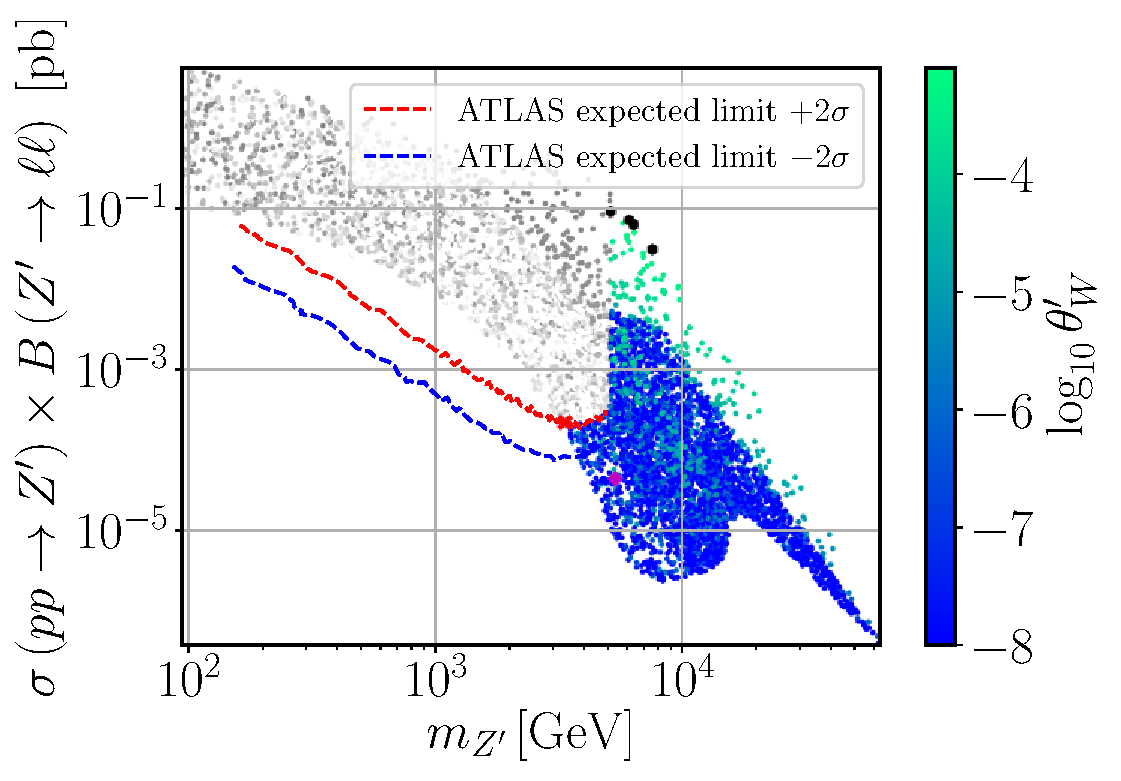
\includegraphics[scale=0.27
	]{mZp_Xsec_twp.pdf}~
	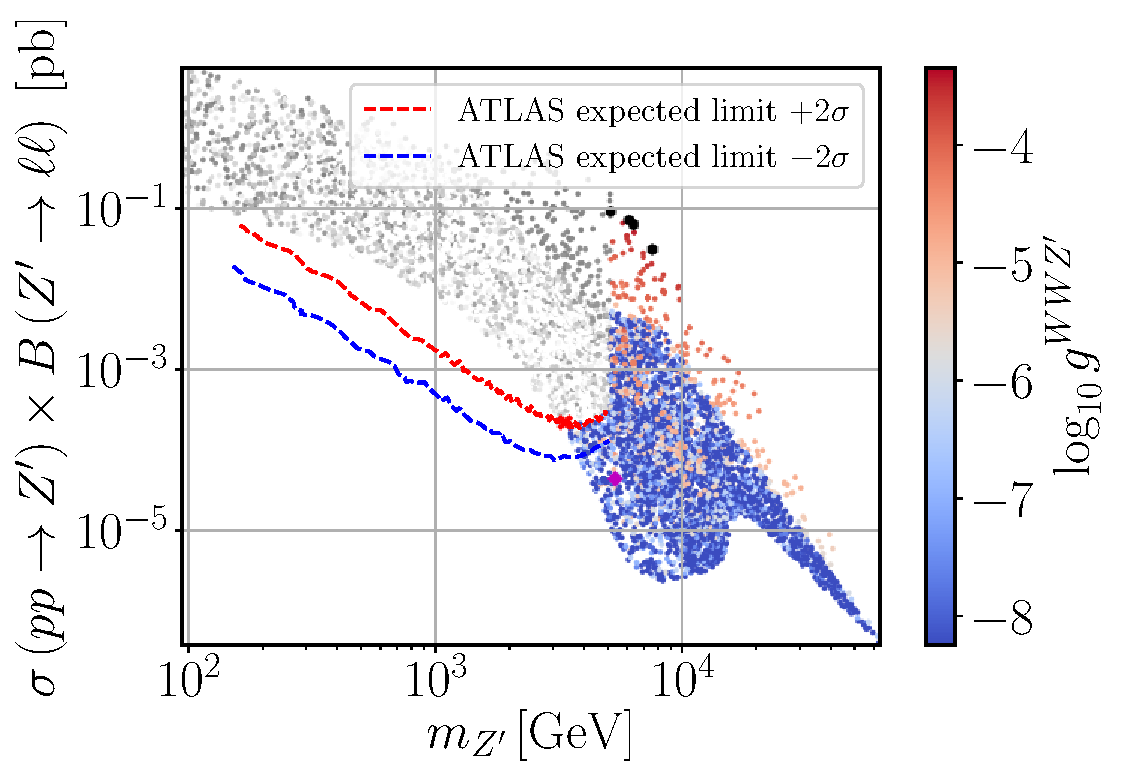
\includegraphics[scale=0.27
]{mZp_Xsec_gWWZp.pdf}	
\end{figure}	
%%%%%%%%%%%%%%%%%%%%%%%%%
Small coupling of $Z'$ to $W$ bosons: $g^{WWZ^\prime} \simeq \dfrac{1}{16} \dfrac{\g{YB}{}}{\g{B-L}{}} \(\dfrac{v}{x}\)^2\,.$
\end{frame}

\begin{frame}
Two-loop Barr-Zee type contributions are subdominant
%%%%%%%%%%%%%%%%%%%%%%%%%
\begin{figure}[!h]
	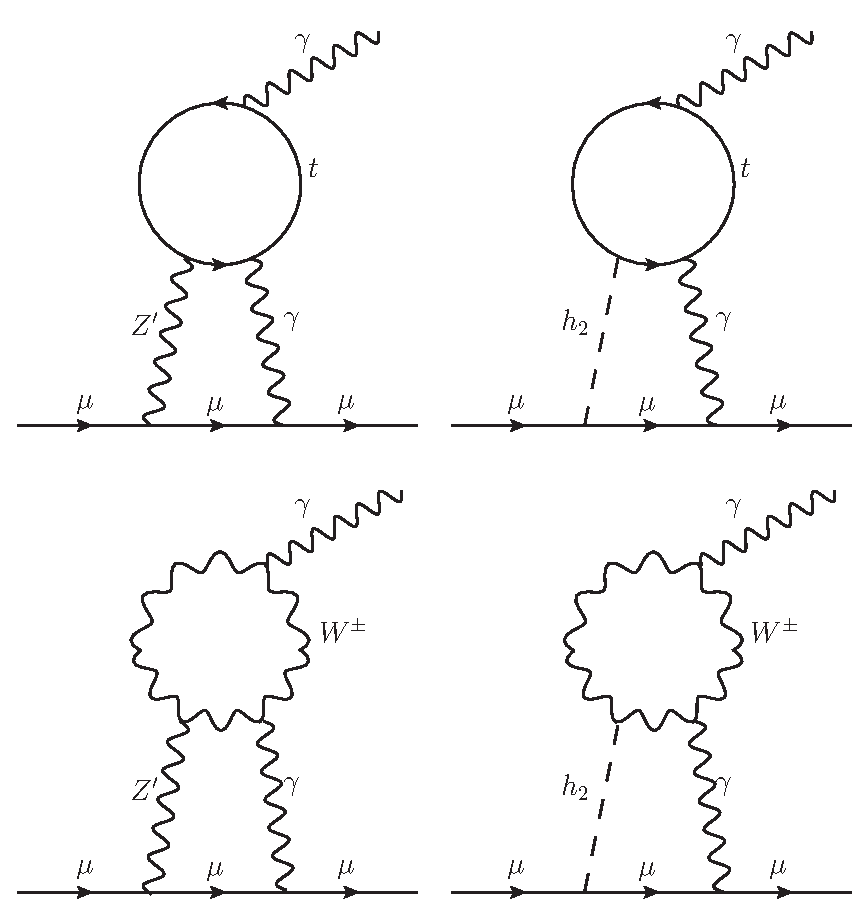
\includegraphics[scale=0.32
	]{Barr-Zee.pdf}
\end{figure}	
%%%%%%%%%%%%%%%%%%%%%%%%%
Larger contribution	from the top-left diagram due to $\g{L,R}{ttZ'} \gg \g{}{WWZ'}, \alpha_h$, however:
\begin{equation*}
\dfrac{\Delta a_\mu^{\text{Barr-Zee}}}{\Delta a_\mu^{Z^\prime}} \simeq -\dfrac{1}{65536 \pi^2}\dfrac{g^2 \(g^2 + \g{Y}{2}\) \g{YB}{3}}{\[3 \g{B-L}{} \g{YB}{}  + 2\(\g{B-L}{2} + \g{YB}{2} \) \] } \(\dfrac{v}{x}\)^4 \ll 1 
\end{equation*}

\end{frame}

\begin{frame}{Benchmark points}
	%
	\begin{table}[htb!]
		\begin{center}
			\resizebox{\columnwidth}{!}{%
				%\begin{ruledtabular}
				\begin{tabular}{ccccccccccc}
					\toprule                     
					$m_{Z^\prime}$ & $m_{h_2}$ &  $x$& $ \log_{10} \Delta a_\mu^\mathrm{NP}$ & $\sigma B$ & $\theta_W^\prime$ & $\alpha_h$ & $\g{B-L}{}$ & $\g{YB}{}$ & $ \g{L}{\ell \ell Z^\prime}$ & $\g{R}{\ell \ell Z^\prime}$ \vspace{1mm}
					\\
					\hline \vspace{-2mm} \\ 
					%%%%%%%%%%
					$3.13$ 			    							& $3.72$ 			    				& $15.7$		& $-12.1$	&	$2.22\times 10^{-4}$ &	$\approx 0$ &	$5.67 \times 10^{-5}$ &	$0.0976$ &	$2.0 \times 10^{-8}$ &	$0.0976$ &	$0.0976$\vspace{1mm} 	\\
					%%%%%%%%%%
					$5.37$ 			    							& $0.396$ 			    				& $9.10$		& $-11.7$	&	$4.23 \times 10^{-5}$ &	$2.55 \times 10^{-7}$ &	$9.44 \times 10^{-7}$ &	$0.302$ &	$8.73 \times 10^{-4}$ &	$0.302$ &	$0.303$\vspace{1mm}  	\\
					%%%%%%%%%%
					$7.59$ 			    							& $3.072$ 			    				& $4.36$		& $-9.89$	&	$0.0302$ &	$7.26 \times 10^{-4}$ &	$0.0471$ &	$0.612$ &	$1.99$ &	$3.37$ &	$2.76$\vspace{1mm}  	\\
					%%%%%%%%%%
					$6.13$ 			    							& $2.24$ 			    				& $6.67$		& $-9.92$	&	$0.0696$ &	$8.0 \times 10^{-4}$ &	$0.0593 $ &	$0.383$ &	$2.80$ &	$1.78$ &	$3.18$ \vspace{1mm}  	\\
					%%%%%%%%%%
					$6.373$ 			    							& $3.43$ 			    				& $6.56$		& $-9.92$	&	$0.0615$ &	$7.86 \times 10^{-4}$ &	$0.0266 $ &	$0.395$ &	$2.82$ &	$1.81$ &	$3.22$ \vspace{1mm}  	\\
					%%%%%%%%%%
					$5.14$ 			    							& $4.21$ 			    				& $2.77$		& $-9.94$	&	$0.0896$ &	$6.52 \times 10^{-4}$ &	$0.0132 $ &	$0.871$ &	$1.86$ &	$1.80$ &	$2.73$ \vspace{1mm}  	\\
					\bottomrule
				\end{tabular}
				%		\end{ruledtabular}
			}
		\end{center}
	\end{table}
	% 
	\vskip4mm
	\begin{itemize}
		\item \textbf{First line:} Early discovery/exclusion scenario with the lightest $Z'$ found in the scan,
		\vskip2mm
		\item \textbf{Second line:} Lightest new scalar found in the scan,
		\vskip2mm
		\item \textbf{Third to fourth lines:} Four best $\(g-2\)_\mu$ points. 
	\end{itemize}
\end{frame}


\section{Conclusions and outlook}

\begin{frame}{Conclusions and outlook}
	\textbf{\purple Muon $\(g-2\)_\mu$ anomaly:}
\begin{itemize}
	\item A heavy $Z'$ between $5$ and $8~\mathrm{TeV}$ can explain it up to a $2.25\sigma$ uncertainty,
	\item Needs sizeable kinetic-mixing parameter $\g{YB}{}$
\end{itemize}
\vskip2mm
	\textbf{\purple New physics searches}
\begin{itemize}
	\item We have identified 6 benchmark points to test the B-L SM at future LHC searches:
	\vskip2mm
	\begin{itemize}
		\item For a relatively light new scalar, $m_{h_2} \approx 400~\mathrm{GeV}$
		\vskip1mm
		\item For an early discovery/exclusion $Z'$ boson $m_{Z'} \approx 3.1~\mathrm{TeV}$
		\vskip1mm
		\item For maximal contribution to the muon $\(g-2\)_\mu$ anomaly
	\end{itemize} 
\end{itemize}
\end{frame}


\end{document}
